% ========================================
%	Header einbinden
% ========================================

\documentclass[bibtotoc,titlepage]{scrartcl}

% Deutsche Spracheinstellungen
\usepackage[ngerman,german]{babel, varioref}
\usepackage[T1]{fontenc}
\usepackage[utf8]{inputenc}

%\usepackage{marvosym}

\usepackage{amsfonts}
\usepackage{amssymb}
\usepackage{amsmath}
\usepackage{amscd}
\usepackage{amstext}

\usepackage{longtable}

%\usepackage{bibgerm}

\usepackage{footnpag}

\usepackage{ifthen}                 %%% package for conditionals in TeX
\usepackage[amssymb]{SIunits}
%Für textumflossene Bilder und Tablellen
%\usepackage{floatflt} - veraltet

%Für Testzwecke aktivieren, zeigt labels und refs im Text an.
%\usepackage{showkeys}

% Abstand zwischen zwei Absätzen nach DIN (1,5 Zeilen)
% \setlength{\parskip}{1.5ex plus0.5ex minus0.5ex}

% Einrückung am Anfang eines neuen Absatzes nach DIN (keine)
%\setlength{\parindent}{0pt}

% Ränder definieren
% \setlength{\oddsidemargin}{0.3cm}
% \setlength{\textwidth}{15.6cm}

% bessere Bildunterschriften
%\usepackage[center]{caption2}


% Problemlösungen beim Umgang mit Gleitumgebungen
\usepackage{float}

% Nummeriert bis zur Strukturstufe 3 (also <section>, <subsection> und <subsubsection>)
%\setcounter{secnumdepth}{3}

% Führt das Inhaltsverzeichnis bis zur Strukturstufe 3
%\setcounter{tocdepth}{3}
\usepackage[version=3]{mhchem}
	\mhchemoptions{minus-sidebearing-left=0.06em, minus-sidebearing-right=0.11em}
\usepackage{exscale}

\newenvironment{dsm} {\begin{displaymath}} {\end{displaymath}}
\newenvironment{vars} {\begin{center}\scriptsize} {\normalsize \end{center}}


\newcommand {\en} {\varepsilon_0}               % Epsilon-Null aus der Elektrodynamik
\newcommand {\lap} {\; \mathbf{\Delta}}         % Laplace-Operator
\newcommand {\R} { \mathbb{R} }                 % Menge der reellen Zahlen
\newcommand {\e} { \ \mathbf{e} }               % Eulersche Zahl
\renewcommand {\i} { \mathbf{i} }               % komplexe Zahl i
\newcommand {\N} { \mathbb{N} }                 % Menge der nat. Zahlen
\newcommand {\C} { \mathbb{C} }                 % Menge der kompl. Zahlen
\newcommand {\Z} { \mathbb{Z} }                 % Menge der kompl. Zahlen
\newcommand {\limi}[1]{\lim_{#1 \rightarrow \infty}} % Limes unendlich
\newcommand {\sumi}[1]{\sum_{#1=0}^\infty}
\newcommand {\rot} {\; \mathrm{rot} \,}         % Rotation
\newcommand {\grad} {\; \mathrm{grad} \,}       % Gradient
\newcommand {\dive} {\; \mathrm{div} \,}        % Divergenz
\newcommand {\dx} {\; \mathrm{d} }              % Differential d
\newcommand {\cotanh} {\; \mathrm{cotanh} \,}   %Cotangenshyperbolicus
\newcommand {\asinh} {\; \mathrm{areasinh} \,}  %Area-Sinus-Hyp.
\newcommand {\acosh} {\; \mathrm{areacosh} \,}  %Area-Cosinus-H.
\newcommand {\atanh} {\; \mathrm{areatanh} \,}  %Area Tangens-H.
\newcommand {\acoth} {\; \mathrm{areacoth} \,}  % Area-cotangens
\newcommand {\Sp} {\; \mathrm{Sp} \,}
\newcommand {\mbe} {\stackrel{\text{!}}{=}}     %Must Be Equal
\newcommand{\qed} { \hfill $\square$\\}
\renewcommand{\i} {\imath}
\def\captionsngerman{\def\figurename{\textbf{Abb.}}}

%%%%%%%%%%%%%%%%%%%%%%%%%%%%%%%%%%%%%%%%%%%%%%%%%%%%%%%%%%%%%%%%%%%%%%%%%%%%
% SWITCH FOR PDFLATEX or LATEX
%%%%%%%%%%%%%%%%%%%%%%%%%%%%%%%%%%%%%%%%%%%%%%%%%%%%%%%%%%%%%%%%%%%%%%%%%%%%
%%%
\ifx\pdfoutput\undefined %%%%%%%%%%%%%%%%%%%%%%%%%%%%%%%%%%%%%%%%% LATEX %%%
%%%
\usepackage[dvips]{graphicx}       %%% graphics for dvips
\DeclareGraphicsExtensions{.eps,.ps}   %%% standard extension for included graphics
\usepackage[ps2pdf]{thumbpdf}      %%% thumbnails for ps2pdf
\usepackage[ps2pdf,                %%% hyper-references for ps2pdf
bookmarks=true,%                   %%% generate bookmarks ...
bookmarksnumbered=true,%           %%% ... with numbers
hypertexnames=false,%              %%% needed for correct links to figures !!!
breaklinks=true,%                  %%% breaks lines, but links are very small
linkbordercolor={0 0 1},%          %%% blue frames around links
pdfborder={0 0 112.0}]{hyperref}%  %%% border-width of frames
%                                      will be multiplied with 0.009 by ps2pdf
%
\hypersetup{ pdfauthor   = {Hannes Franke; Julius Tilly},
pdftitle    = {V301 Innenwiderstand und Leistungsanpassung}, pdfsubject  = {Protokoll FP}, pdfkeywords = {V301, Innenwiderstand, Leistungsanpassung},
pdfcreator  = {LaTeX with hyperref package}, pdfproducer = {dvips
+ ps2pdf} }
%%%
\else %%%%%%%%%%%%%%%%%%%%%%%%%%%%%%%%%%%%%%%%%%%%%%%%%%%%%%%%%% PDFLATEX %%%
%%%
\usepackage[pdftex]{graphicx}      %%% graphics for pdfLaTeX
\DeclareGraphicsExtensions{.pdf}   %%% standard extension for included graphics
\usepackage[pdftex]{thumbpdf}      %%% thumbnails for pdflatex
\usepackage[pdftex,                %%% hyper-references for pdflatex
bookmarks=true,%                   %%% generate bookmarks ...
bookmarksnumbered=true,%           %%% ... with numbers
hypertexnames=false,%              %%% needed for correct links to figures !!!
breaklinks=true,%                  %%% break links if exceeding a single line
linkbordercolor={0 0 1},
linktocpage]{hyperref} %%% blue frames around links
%                                  %%% pdfborder={0 0 1} is the default
\hypersetup{
pdftitle    = {V301 Innenwiderstand und Leistungsanpassung}, 
pdfsubject  = {Protokoll AP}, 
pdfkeywords = {V301, Innenwiderstand, Leistungsanpassung},
pdfsubject  = {Protokoll AP},
pdfkeywords = {V301, Innenwiderstand, Leistungsanpassung}}
%                                  %%% pdfcreator, pdfproducer,
%                                      and CreationDate are automatically set
%                                      by pdflatex !!!
\pdfadjustspacing=1                %%% force LaTeX-like character spacing
\usepackage{epstopdf}
%
\fi %%%%%%%%%%%%%%%%%%%%%%%%%%%%%%%%%%%%%%%%%%%%%%%%%%% END OF CONDITION %%%
%%%%%%%%%%%%%%%%%%%%%%%%%%%%%%%%%%%%%%%%%%%%%%%%%%%%%%%%%%%%%%%%%%%%%%%%%%%%
% seitliche Tabellen und Abbildungen
%\usepackage{rotating}
\usepackage{ae}
\usepackage{
  array,
  booktabs,
  dcolumn
}
\makeatletter 
  \renewenvironment{figure}[1][] {% 
    \ifthenelse{\equal{#1}{}}{% 
      \@float{figure} 
    }{% 
      \@float{figure}[#1]% 
    }% 
    \centering 
  }{% 
    \end@float 
  } 
  \makeatother 


  \makeatletter 
  \renewenvironment{table}[1][] {% 
    \ifthenelse{\equal{#1}{}}{% 
      \@float{table} 
    }{% 
      \@float{table}[#1]% 
    }% 
    \centering 
  }{% 
    \end@float 
  } 
  \makeatother 
%\usepackage{listings}
%\lstloadlanguages{[Visual]Basic}
%\allowdisplaybreaks[1]
%\usepackage{hycap}
%\usepackage{fancyunits}


% ========================================
%	Angaben für das Titelblatt
% ========================================

\title{Versuch 606 - Messung des Suszeptibilität paramagnetischer Substanzen\\				% Titel des Versuchs 
\large TU Dortmund, Fakultät Physik\\ 
\normalsize Anfänger-Praktikum}

\author{Jan Adam\\			% Name Praktikumspartner A
{\small \href{jan.adam@tu-dortmund.de}{jan.adam@tu-dortmund.de}}	% Erzeugt interaktiven einen Link
\and						% um einen weiteren Author hinzuzfügen
Dimitrios Skodras\\					% Name Praktikumspartner B
{\small \href{dimitrios.skodras@tu-dortmund.de}{dimitrios.skodras@tu-dortmund.de}}		% Erzeugt interaktiven einen Link
}
\date{09.April2013}				% Das Datum der Versuchsdurchführung

% ========================================
%	Das Dokument beginnt
% ========================================

\begin{document}

% ========================================
%	Titelblatt erzeugen
% ========================================

\maketitle					% Jetzt wird die Titelseite erzeugt
\thispagestyle{empty} 				% Weder Kopfzeile noch Fußzeile

% ========================================
%	Der Vorspann
% ========================================

%\newpage					% Wenn Verzeichnisse auf einer neuen Seite beginnen sollen
%\pagestyle{empty}				% Weder Kopf- noch Fußzeile für Verzeichnisse

\tableofcontents

%\newpage					% eine neue Seite
%\thispagestyle{empty}				% Weder Kopf- noch Fußzeile für Verzeichnisse
%\listoffigures					% Abbildungsverzeichnis

%\newpage					% eine neue Seite
%\thispagestyle{empty}				% Weder Kopf- noch Fußzeile für Verzeichnisse
%\listoftables					% Tabellenverzeichnis
\newpage					% eine neue Seite


% ========================================
%	Kapitel
% ========================================

\section{Theorie}
\setcounter{page}{1}
\subsection{Die magnetische Suszeptibilität}
Die magnetische Suszeptibilität $\chi$ ist eine physikalische Größe, die den Einfluss eines externen Magnetfelds $\vec B$ auf
die Magnetisierbarkeit eines Substanz beschreibt. Sie ist kompliziert von der magnetischen Feldstärke $\vec H$ und der Temperatur $T$
abhängig. Auch in der Relation von magnetischer Flussdichte und magnetischer Feldstärke 
\begin{align}
 \vec B = \mu_0 \vec H + \vec M
\end{align}
tritt sie auf, wobei $\vec M$ die Magnetisierung ist und durch atomare magnetische Momente einer Probe entsteht und mit $\chi$ verknüpft ist
\begin{align}
 \vec M = N \mu_0 \,  \bar{\vec{\mu}} =\mu_0 \chi \vec H.
 \label{eqMagnetisierung}
\end{align}

Im Gegensatz zum Diamagnetismus, der die Induktion eines Magnetfelds antiparallel zum Außenfeld beschreibt, handelt es sich beim
Phänomen des Paramagnetismus um die Induktion eines Magnetfeld, das sich parallel ausrichtet. Diese Eigenschaft ist nur bei Stoffen
zu finden, die einen von Null verschiedenen Drehimpuls haben. Dieser Drehimpuls hängt mit den zum Außenfeld relativen, magnetischen 
Momenten zusammen.

\subsection{Berechnung der magnetischen Suszeptibilität}
Der Drehimpuls $\vec J$ setzt sich durch Vektorsummation aus dem Bahndrehimpuls der Elektronenhülle $\vec L$ und dem Eigendrehimpuls der Elektronen 
$\vec S$ zusammen. Die Beträge der zugehörigen magnetischen Momente ergeben sich aus der Quantenmechanik zu

\begin{align}
 | \mu_L | = \mu_B \sqrt{L(L+1)} \qquad \text{und} \qquad |\mu_S| = \mu_B \, g_S \sqrt{S(S+1)}.
\end{align}

$\mu_B$ ist hierbei das Bohrsche Magneton und $g_S$ das gyromagnetische Verhältnis des freien Elektrons. Das magnetische Moment zum
Gesamtdrehimpuls $\mu_J$ ergibt sich über Winkelbeziehungen der Zwischenwinkel der beiden Vektoren $\mu_L$ und $\mu_S$ zu dem Ausdruck

\begin{align}
 |\mu_J| \approx \mu_B \, g_J \sqrt{J(J+1)}, \intertext{mit $g_J$ als Landé-Faktor}  g_J = \frac{3J(J+1)\, + \, \{S(S+1) + L(L+1)\}}{2J(J+1)}.
 \label{eq_lande}
\end{align}

Besagte Winkel sind allerdings nicht beliebig. Das Phänomen der Richtungsquantelung lässt $2J+1$ Orientierungen zu. Um die Magnetisierung
nun zu berechnen, wird die Häufigkeit jeder Orientierung ermittelt, mit dem zugehörigen Betrag des magnetischen Moments $\mu_J$ multipliziert
und aufsummiert. Die Häufigkeitsverteilung $Z(E,T)$ ist hierbei Boltzmann-verteilt

\begin{equation}
 Z(E,T) = \exp \left(-\frac{E}{kT}\right) = \exp\left(-\frac{\mu_B\,g_J\,m\,B}{kT}\right).
\end{equation}

Das in Gleichung \eqref{eqMagnetisierung} aufgeführte mittlere magnetische Moment $\bar{\vec{\mu}}$ ergibt sich aus der Brillouin-Funktion 
von der Boltzmann-Verteilung. Dieser komplizierte Ausdruck wird um Null mit der Taylor-Entwicklung genähert, da das Argument deutlich 
kleiner als Eins ist. Somit ergibt sich der endgültige Ausdruck, welcher dem Curie-Gesetz für große Temperaturen genügt, für die 
magnetische Suszeptibilität zu

\begin{align}
\chi = \frac{\mu_0\,\mu_B^2\,g_J^2\,N\,J(J+1)}{3\,kT}. 
\end{align}

Allerdings ist der Gesamtdrehimpuls J hierbei widerspruchsfrei zu den Hundschen Regeln zu ermitteln. Sie basieren auf der elektrostatischen
Abstoßung der Hüllenelektronen und lauten im einzelnen:

\begin{enumerate}
 \item Die Spins $\vec s_i$ kombinieren sich zum maximalen Gesamtspin $\vec S = \sum \vec s_i$, der nach dem Pauli-Prinzip möglich ist.
 \item Die Bahndrehimpulse $\vec l_i$ setzen sich so zusammen, dass der maximale Drehimpuls $\vec L = \sum \vec l_i$ entsteht, der
 mit dem Pauli-Prinzip und der ersten Regel verträglich ist.
 \item Der Gesamtdrehimpuls ist $\vec J = \vec L - \vec S$, wenn die Schale weniger als halb und $\vec J = \vec L + \vec S$, wenn sie
 mehr als halb gefüllt ist
\end{enumerate}

\subsection{Apparatur zur Messung der Suszeptibilität}
Da die Suszeptibilität paramagnetischer Substanzen eines Außenfeld verstärkt, ist es naheliegend zu ihrer Messung Spulen zu verwenden.
Die Induktivität $L_M$ einer Spule mit Länge $l$ und Windungszahl $n$, welche mit einer Probe gefüllt ist, deren Durchmesser $Q$ kleiner 
als der Spulenquerschnitt $F$ ist, ergibt sich zu

\begin{align}
 L_M = L + \Delta L = \mu_0 \frac{n^2 \,F}{l} + \chi \mu_0\frac {n^2 \, Q}{l}
 \label{eqIndu}
\end{align}

Beim Probenquerschnitt $Q$ ist jedoch noch zu beachten, dass die Dichte des oxidierten Stoffs nicht so dicht ist, wie ein Einkristall. 
Daher muss der reale Querschnitt $Q_{real}$ über die Beziehung

\begin{align}
 Q_{real} = \frac{M_p}{L \, \rho_w},
\end{align}

identifiziert werden, mit $M_p$ als Probenmasse und $\rho_w$ als Dichte eines Einkristalls. Um $\Delta L$ zu bestimmen, ist eine hohe
Auflösung für die Induktivitätsmessung nötig. Durch zwei identische Spulen ist das realisierbar, wenn eine mit der Probe gefüllt ist und
beide über eine Brückenschaltung nach Abbildung \ref{picBruecke} verbunden sind.

\begin{figure}[H]
 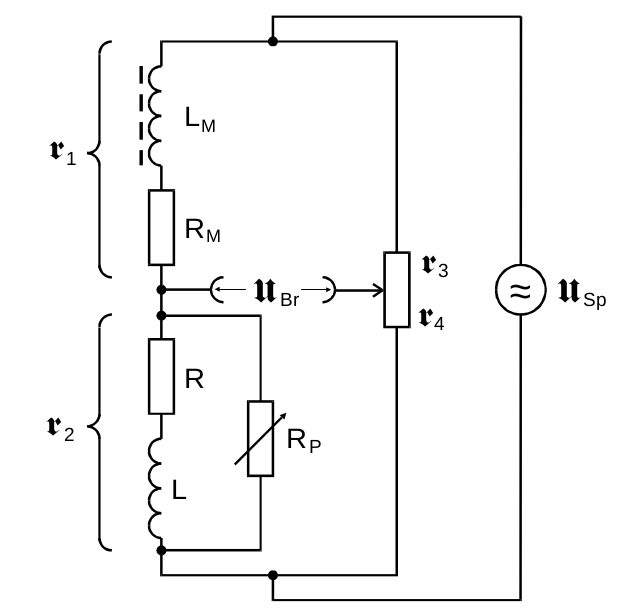
\includegraphics[width=0.7\textwidth]{pics/bruecke.png}
 \caption{Aufbau zur Brückenschaltung (aus Versuchsanleitung)}
 \label{picBruecke}
\end{figure}

Die Brückenspannung $U_{Br}$ hat folgenden Ausdruck

\begin{align}
 U_{Br} = \frac{\omega \Delta L}{4} \frac{1}{\sqrt{R^2+\omega^2L^2}} U_{Sp},
\end{align}

was mit \eqref{eqIndu} und für hohe Frequenzen zur Formel für die Suszeptibilität wird

\begin{align}
 \chi(\omega \to \inf) = 4 \frac{F}{Q} \frac{U_{Br}}{U_{Sp}}.
\end{align}

Die Abgleichbedingung für die Brücke mit eingesetzter Probe errechnet sich zu 

\begin{align}
 \chi = 2 \frac{\Delta R}{r_3} \frac{F}{Q}.
\end{align}

\section{Durchführung}
\subsection{Ermittlung der Filterkurve des Selektiv-Verstärkers}
Die Messung der für die Berechnung der Suszeptibilität nötigen Brückenspannung wird durch die immer vorhandene Störspannung durch
die Außenklemmen der Brückenspannung erschwert. Abhilfe für dieses Problem bietet der Selektiv-Verstärker, dessen gesuchte Filterkurve
wie in Abbildung \ref{picfilter} die Gestalt einer Glockenkurve hat. 

\begin{figure}[H]
 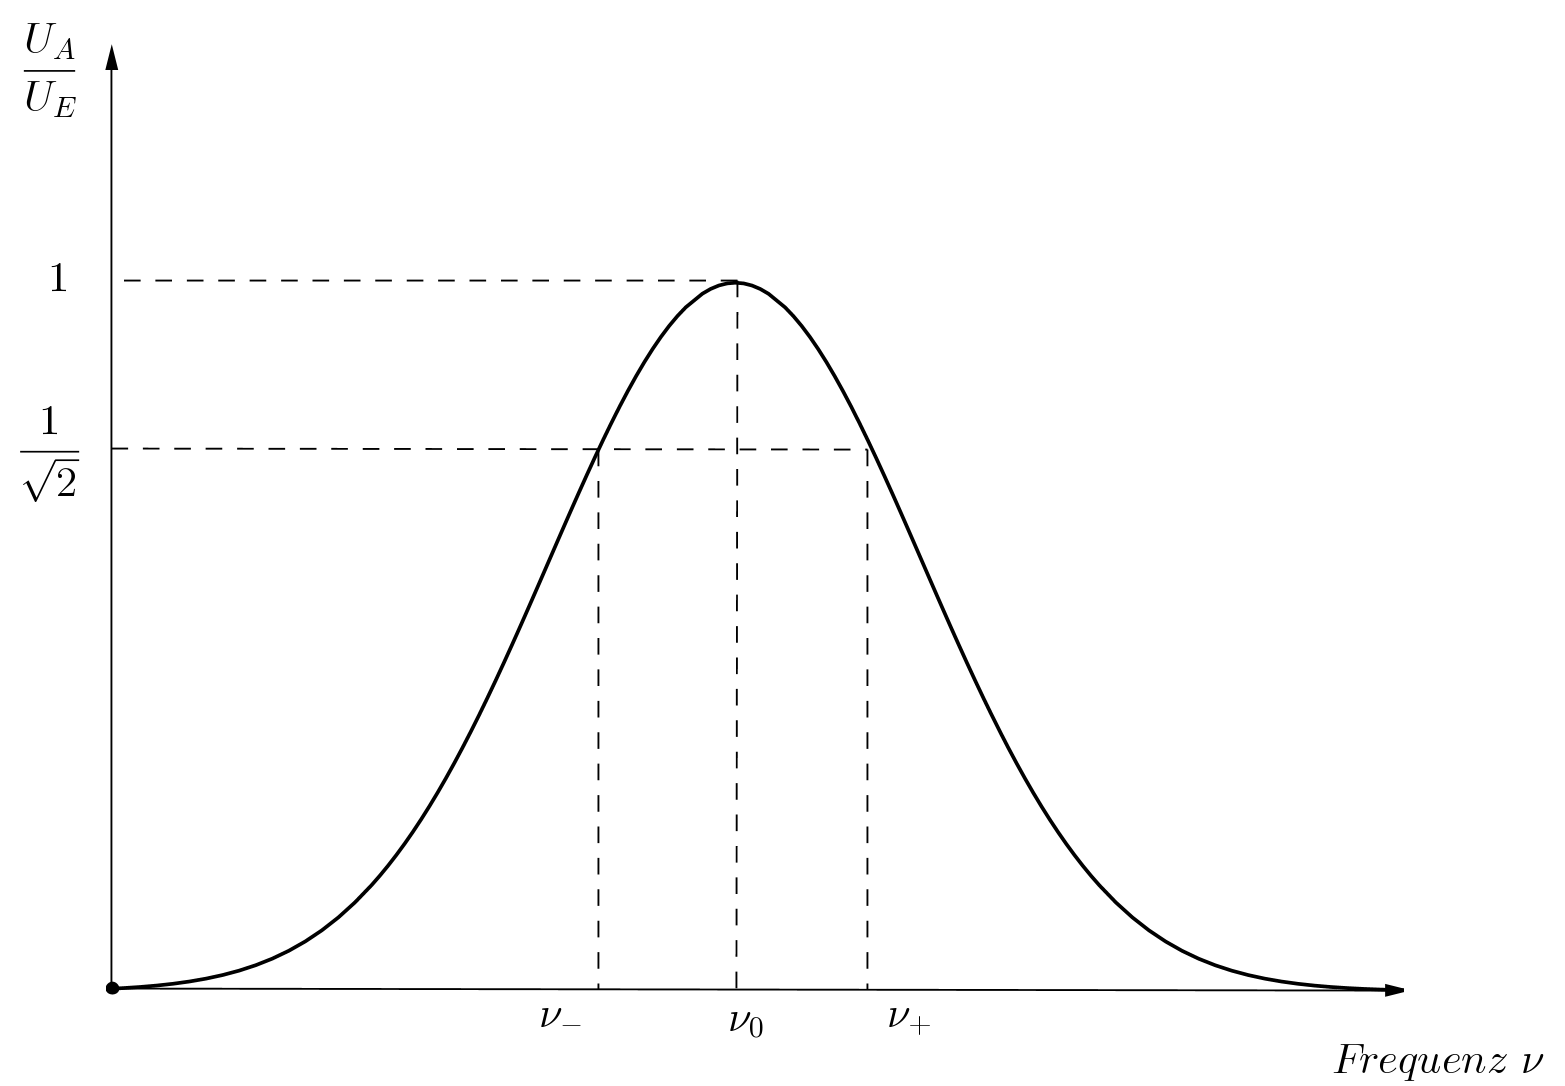
\includegraphics[width=0.8\textwidth]{pics/filterkurve.png}
 \caption{Filterkurve eines Selektiv-Verstärkers}
 \label{picfilter}
\end{figure}

Den Quotienten aus Durchlassfrequenz und der Differenz von $\nu_-$ und $\nu_+$, bei der ein Verhältnis von $1/\sqrt{2}$ bezüglich der 
Spannungen $U_A$ und $U_E$ auftritt, nennt man die Güte $Q$.

Um die Filterkurve nun zu ermitteln, wird ein Sinusgenerator mit einer Effektivspannung von $U_{eff}$ = 1 V in einem Frequenzbereich 
zwischen 20 und 40 kHz betrieben. Die Brückenschaltung wird damit gespeist und nach Vorverstärkungen der geringen Ausgangsspannung,
wird ihr Wert auf einem Millivoltmeter in Abhängigkeit der verwandten Frequenz angezeigt.

\subsection{Messung der Suszeptibilität}
Zu Beginn wird die Durchlassfrequenz des Selektiv-Verstärkers auf die Signalfrequenz eingestellt, die man zuvor als Frequenz zur maximalen
Ausgangsspannung gefunden hat, und gleicht die noch leere Brückenschaltung auf nahe 0 mV ab. Nun wird eine Probe eingeführt und die
neue Brückenspannung gemessen. Zuletzt wird die Brücke erneut abgeglichen und der Wert von $\Delta R$ notiert. 

\section{Auswertung}
Die Suszeptibilität kann zunächst theoretisch nach Modellen der Quantenmechanik bestimmt werden
Für Neodym \ce{Nd_2O_3}\\
Neodym hat 4 Elektronen auf der 4f Schale. Nach abzug der 3 Elektronen für die Oxidbindung verbleiben noch 3. Der Gesamtspin S beträgt in diesem Fall $\frac{1}{2}+ \frac{1}{2}+ \frac{1}{2} = 1 \frac{1}{2}$\\
Die Hauptquantenzahl ist maximal 3. Folglich ergibt sich für den Gesamtdrehimpuls $3+2+1=6$.\\
Da die Schale zu weniger als die Hälfte befüllt ist, errechnet sich der Gesamtimpuls zu $J=|L-S|=4,5$\\
Nach Formel \eqref{eq_lande} ergibt sich:
\begin{align}
g_J=\frac{3\cdot4,5\cdot5,5+[1,5\cdot2,5-6\cdot7]}{2\cdot 3,5\cdot4,5}=0,73
\end{align}

Für Gadolinium \ce{Gd_2O_3}\\
Gadolinium hat 7 Elektronen auf der 4f Schale. Nach abzug der 3 Elektronen für die Oxidbindung verbleiben immer noch 7. Der Gesamtspin S beträgt in diesem Fall $7\cdot\frac{1}{2} = 3,5$\\
Die Hauptquantenzahl ist maximal 3. Folglich ergibt sich für den Gesamtdrehimpuls $3+2+1+0-1-2-3=0$.\\
Da die Schale genau zur Hälfte befüllt ist, errechnet sich der Gesamtimpuls beliebig zu $J=|L-S|=L+S=3,5$\\
Nach Formel \eqref{eq_lande} ergibt sich:
\begin{align}
g_J=\frac{3\cdot3,5\cdot4,5+3,5\cdot4,5}{2\cdot 3,5\cdot4,5}=2
\end{align}

Für Dysprosium \ce{Dy_2O_3}\\
Dysprosium hat 10 Elektronen auf der 4f Schale. Nach abzug der 3 Elektronen für die Oxidbindung verbleiben noch 9. Der Gesamtspin S beträgt in diesem Fall $7\cdot \frac{1}{2}-2\cdot\frac{1}{2}= 2 \frac{1}{2}$\\
Die Hauptquantenzahl ist maximal 3. Folglich ergibt sich für den Gesamtdrehimpuls $3+2+1+0-1-2-3+3+2=5$.\\
Da die Schale zu mehr als die Hälfte befüllt ist, errechnet sich der Gesamtimpuls zu $J=L+S=7,5$\\
Nach Formel \eqref{eq_lande} ergibt sich:
\begin{align}
g_J=\frac{3\cdot7,5\cdot8,5+[2,5\cdot3,5-7,5\cdot8,5]}{2\cdot 7,5\cdot8,5}=1,07
\end{align}
\section{Diskussion}

% ========================================
%	Literaturverzeichnis
% ========================================

%\bibliographystyle{plainnat}			% Bibliographie-Style auswählen
%\bibliography{BIBDATEI}			% Literaturverzeichnis

% ========================================
%	Das Dokument endent
% ========================================

\end{document}
